\documentclass[12pt,a4paper]{report}

% Packages
\usepackage[utf8]{inputenc}
\usepackage[margin=1in]{geometry}
\usepackage{amsmath,amssymb,amsfonts}
\usepackage{graphicx}
\usepackage{booktabs}
\usepackage{tabularx}
\usepackage{xcolor}
\usepackage{hyperref}
\usepackage{fancyhdr}
\usepackage{titlesec}
\usepackage{microtype}
\usepackage{float}
\usepackage{caption}
\usepackage{subcaption}

\hypersetup{
    colorlinks=true,
    linkcolor=teal,
    citecolor=blue,
    urlcolor=teal,
    pdftitle={NLP-Based Academic Information Retrieval System},
    pdfauthor={KUET CSE Students}
}

% Header and Footer
\setlength{\headheight}{15pt}
\pagestyle{fancy}
\fancyhf{}
\fancyhead[L]{\small\nouppercase{\leftmark}}
\fancyhead[R]{\small CSE 4122: NLP Lab Final Project}
\fancyfoot[C]{\thepage}
\renewcommand{\headrulewidth}{0.4pt}
\renewcommand{\footrulewidth}{0.2pt}

% Title Formatting
\titleformat{\chapter}[display]
  {\normalfont\bfseries\color{teal}}
  {\filleft\Large\chaptertitlename\ \Huge\thechapter}
  {2ex}
  {\titlerule\vspace{2ex}\huge}
  [\vspace{1ex}\titlerule]

\begin{document}

% ---------------------------------------------------------------------------
% TITLE PAGE
% ---------------------------------------------------------------------------
\begin{titlepage}
    \centering
    \vspace*{0.5cm}
    
    {\huge\bfseries\color{teal} Khulna University of Engineering \& Technology\par}
    \vspace{0.4cm}
    {\Large\textbf{Department of Computer Science and Engineering}\par}
    \vspace{1.5cm}
    
    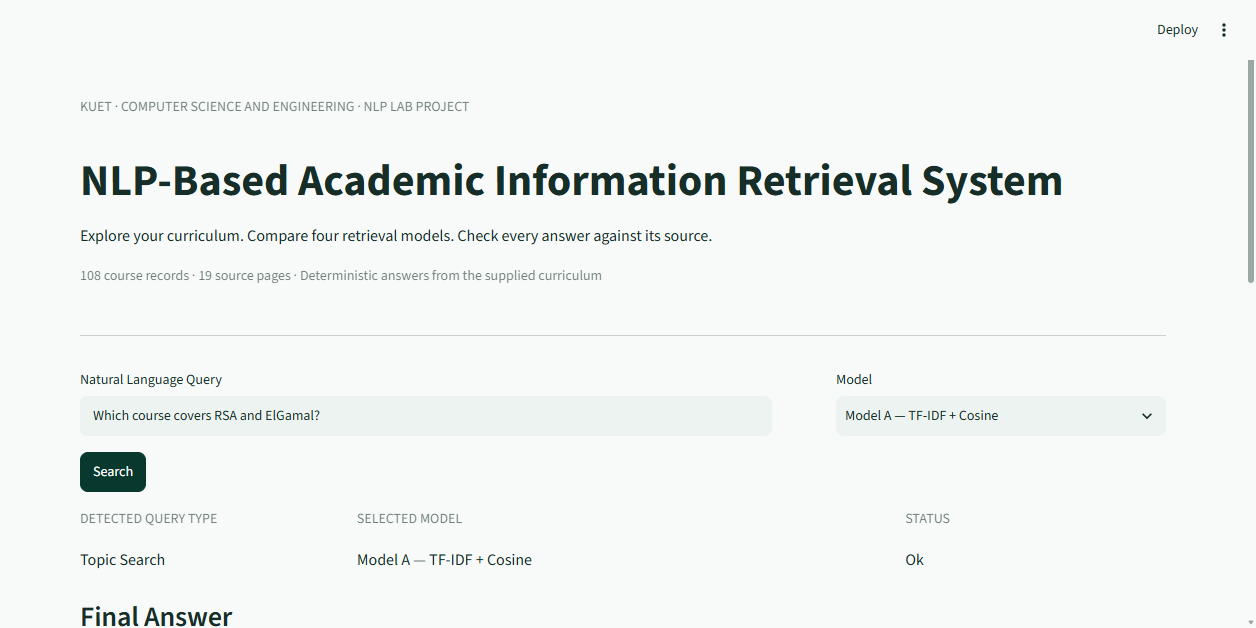
\includegraphics[width=0.25\textwidth]{figures/demo-search.png}\par
    \vspace{1.2cm}
    
    {\Huge\bfseries NLP-Based Academic Information Retrieval System\par}
    \vspace{0.4cm}
    {\large\textit{A Comparative Empirical Study of Lexical, Static Embedding, Deep Recurrent, and Transformer-Based Representations on University Curricula}\par}
    
    \vspace{1.5cm}
    
    {\Large\textbf{CSE 4122: Natural Language Processing Laboratory}\par}
    {\large Final Project Report\par}
    
    \vfill
    
    \begin{minipage}{0.45\textwidth}
        \begin{flushleft}
            \textbf{Submitted By:}\\
            \textit{Department of CSE}\\
            KUET, Khulna-9203
        \end{flushleft}
    \end{minipage}
    \hfill
    \begin{minipage}{0.45\textwidth}
        \begin{flushright}
            \textbf{Course Instructors:}\\
            \textit{Faculty Members}\\
            Department of CSE, KUET
        \end{flushright}
    \end{minipage}
    
    \vspace{1.2cm}
    {\large Academic Year: 2026\par}
    {\small Date of Submission: September 2026\par}
\end{titlepage}

% ---------------------------------------------------------------------------
% ABSTRACT
% ---------------------------------------------------------------------------
\pagenumbering{roman}
\chapter*{Abstract}
\addcontentsline{toc}{chapter}{Abstract}

Traditional search over university curriculum documentation is dominated either by simplistic keyword lookup or by unconstrained generative large language models (LLMs) that frequently hallucinate course credits, prerequisites, and syllabi. This report presents the design, end-to-end implementation, and empirical evaluation of the \textbf{NLP-Based Academic Information Retrieval (IR) System}, an open-source, zero-hallucination semantic search application engineered over the official undergraduate curriculum of the Department of Computer Science and Engineering, Khulna University of Engineering \& Technology (KUET).

Strictly adhering to academic integrity constraints, the system disallows external generative APIs, retrieval-augmented generation (RAG) synthesis, or synthetic answer invention. Instead, it formulates academic query answering through structured document retrieval grounded in 108 extracted course records from a 19-page curriculum PDF. The project synthesizes the core themes of five foundational laboratory modules: (1) lexical preprocessing, lemmatization, and Levenshtein typo-correction (Lab~1); (2) sublinear TF-IDF with $N$-gram representations and vector space cosine similarity (Lab~2); (3) pretrained Word2Vec with TF-IDF weighted document embedding (Lab~3); (4) dynamic token embeddings fed into a Siamese Bidirectional Long Short-Term Memory (BiLSTM) supervised relevance classifier (Lab~4); and (5) contextual sentence transformer embeddings using Sentence-BERT (\texttt{all-MiniLM-L6-v2}) (Lab~5).

Using a rigorously audited held-out benchmark of 48 queries spanning exact, semantic, typo-infused, ambiguous, metadata, and out-of-domain categories, we evaluate each representation across standard IR metrics: Hit@1, Hit@3, Mean Reciprocal Rank (MRR), Recall@3, and Out-of-Domain (OOD) rejection accuracy. SBERT achieves the strongest overall ranking (Hit@1 of 77.8\%, MRR of 0.818), while TF-IDF excels at keyword terminology (Hit@3 of 91.7\%). Model~C (BiLSTM) demonstrates significant overfitting on small-sample query-course pairs (Hit@1 of 5.6\%), providing a critical empirical lesson on the limitations of deep supervised models under limited annotated data. Finally, an interactive Streamlit application exposes real-time side-by-side model comparisons, explainable similarity scores, and verbatim source page provenance.

\vspace{1cm}
\noindent\textbf{Keywords:} Academic Information Retrieval, Natural Language Processing, TF-IDF, Word2Vec, BiLSTM, Sentence-BERT, Rejection Thresholds, Zero Hallucination.

\newpage
\tableofcontents
\listoffigures
\listoftables

% ---------------------------------------------------------------------------
% CHAPTER 1: INTRODUCTION
% ---------------------------------------------------------------------------
\clearpage
\pagenumbering{arabic}
\chapter{Introduction}

\section{Background and Motivation}
Academic curricula in higher education institutions are typically disseminated as lengthy, multi-page PDF documents. At Khulna University of Engineering \& Technology (KUET), the Department of Computer Science and Engineering issues its official undergraduate syllabus as a comprehensive document specifying course codes, credit allocations, contact hours, weekly distributions, and detailed topic outlines.

Students, faculty members, and academic advisors frequently need to query this repository for critical information:
\begin{itemize}
    \item \textbf{Topic discovery:} \textit{``Which subject teaches asymmetric cryptography and RSA?''}
    \item \textbf{Administrative inquiries:} \textit{``How many credits does Natural Language Processing have?''}
    \item \textbf{Term planning:} \textit{``Which laboratory courses are in the 4th year 1st term?''}
    \item \textbf{Prerequisite \& lab cross-referencing:} \textit{``Does CSE 4115 have an accompanying sessional?''}
\end{itemize}

Manual inspection of a 19-page tabular and descriptive syllabus is slow and prone to oversight. While modern generative conversational agents (e.g., ChatGPT, Claude) can respond to natural language questions, they suffer from severe hallucination when applied to specific institutional documents. They frequently invent course codes, misstate credit allocations, or assert prerequisites that do not exist in the official syllabus. 

\section{Project Objectives}
The primary objective of this project is to build an accurate, transparent, and completely local \textbf{Academic Information Retrieval System} based on the supplied KUET CSE curriculum. 

The core research and engineering objectives are:
\begin{enumerate}
    \item Parse the curriculum PDF course-by-course, extracting structured metadata, physical page provenance, and syllabus descriptions into an indexed corpus.
    \item Implement and benchmark four distinct generations of NLP retrieval paradigms on the exact same corpus:
    \begin{itemize}
        \item \textbf{Model A:} Lexical baseline using Term Frequency-Inverse Document Frequency (TF-IDF) and Cosine Similarity.
        \item \textbf{Model B:} Static dense semantic retriever using pretrained Word2Vec embeddings weighted by corpus TF-IDF.
        \item \textbf{Model C:} Deep supervised sequence relevance model using a Siamese Bidirectional LSTM (BiLSTM).
        \item \textbf{Model D:} Pretrained contextual embedding retriever using Sentence-BERT (\texttt{all-MiniLM-L6-v2}).
    \end{itemize}
    \item Develop an intent classification and deterministic answer formatting pipeline that guarantees zero hallucination by returning factual curriculum excerpts with exact page citations.
    \item Provide an interactive, responsive Streamlit dashboard for real-time model comparison, explainable scoring inspection, and instantaneous querying.
\end{enumerate}

\section{Architectural and Negative Constraints}
To ensure academic rigor and evaluate genuine NLP techniques, the project was developed under strict constraints:
\begin{itemize}
    \item \textbf{No Generative LLMs:} No OpenAI, Gemini, Claude, or local generative LLM APIs.
    \item \textbf{No RAG Frameworks:} No LangChain, LlamaIndex, or autonomous agent frameworks.
    \item \textbf{No Hallucination:} The system must never write invented summaries or assert unrecorded academic facts. Every answer must originate from verbatim syllabus records.
    \item \textbf{Model Independence:} The application must function completely locally, even if deep transformer models (Model D) are disabled.
    \item \textbf{Rejection by Default:} Unanswerable, gibberish, or out-of-domain questions must be rejected with calibrated thresholds rather than returning forced false positives.
\end{itemize}

\section{Synthesis of Coursework Laboratories}
This project is formulated as the capstone synthesis of the \textbf{CSE 4122 (Natural Language Processing Laboratory)} curriculum, systematically incorporating the topics taught throughout the semester:
\begin{itemize}
    \item \textbf{Lab 1 (Text Preprocessing and Spelling Correction):} Powers the normalization, technical term preservation, WordNet lemmatization, and Levenshtein edit-distance typo corrector.
    \item \textbf{Lab 2 (Text Representation and N-Gram Modeling):} Directly forms the foundation of Model~A, utilizing $(1, 2)$-gram sublinear TF-IDF vector space modeling and cosine similarity.
    \item \textbf{Lab 3 (Word Embeddings and Classifiers):} Forms the mathematical basis of Model~B, using Google News Word2Vec embeddings with corpus TF-IDF weighted pooling.
    \item \textbf{Lab 4 (PyTorch Sequence Models and BiLSTMs):} Powers Model~C, utilizing a bidirectional PyTorch LSTM with dynamic token embedding sequences, packed padding, and paired classification.
    \item \textbf{Lab 5 (Transformer Sequence Encoders):} Realized in Model~D via a sentence-transformer encoder for contextual similarity retrieval.
\end{itemize}

% ---------------------------------------------------------------------------
% CHAPTER 2: CORPUS EXTRACTION & DATASET ENGINEERING
% ---------------------------------------------------------------------------
\chapter{Corpus Extraction and Dataset Engineering}

\section{Source Document Profile}
The raw dataset consists of the official syllabus document: \texttt{CourseContentsCSE\_14\_08\_2022.pdf}. The document is a 19-page PDF covering the four-year undergraduate curriculum effective from the academic session 2021--2022. It comprises summary tables for each term followed by detailed syllabi for theory and laboratory courses.

\section{Automated Extraction Pipeline}
Rather than treating the document as monolithic text, extraction is handled course-by-course using PyMuPDF (\texttt{fitz}) in \texttt{src/corpus/corpus\_builder.py}.

\subsection{Heading Detection and Boundary Extraction}
Courses are detected dynamically using regular expression pattern matching:
\begin{equation}
    \text{Pattern} = \texttt{\textasciicircum([A-Z]\{2,5\})\textbackslash s+(\textbackslash d\{4\})(?:\textbackslash s*:\textbackslash s*|\textbackslash s+)(.+)\$}
\end{equation}
This regex accommodates both standard formatted headings (e.g., \texttt{CSE 4121: Natural Language Processing}) and irregular formatting observed in the official PDF, such as a missing colon in \texttt{CSE 4245 Principles of Programming Languages}.

\subsection{Stateful Metadata Tracking}
As pages are scanned sequentially:
\begin{itemize}
    \item Academic year and term are tracked from section headings (e.g., \textit{``Syllabus of 4th Year 1st Term Courses''}).
    \item Optional group allocations (e.g., \textit{``Optional-I''}, \textit{``Optional-II''}) are preserved to avoid assuming that elective courses are compulsory for all students.
    \item Descriptions continuing across physical page boundaries are stitched together, while summary tables at the start of terms are segmented to prevent tabular contamination of descriptions.
\end{itemize}

\subsection{Corpus Statistics}
The extraction pipeline generates 108 term-specific course records representing 107 unique course codes. Table~\ref{tab:corpus_stats} summarizes the extracted corpus.

\begin{table}[H]
    \centering
    \caption{Summary Statistics of Extracted KUET CSE Corpus}
    \label{tab:corpus_stats}
    \begin{tabularx}{0.85\textwidth}{Xr}
        \toprule
        \textbf{Corpus Metric} & \textbf{Observed Value} \\
        \midrule
        Total Course Records & 108 \\
        Unique Course Codes & 107 \\
        Theory Courses & 64 \\
        Laboratory / Sessional Courses & 40 \\
        Project / Thesis / Seminar Records & 4 \\
        Elective Offerings (Optional Groups I, II, III) & 35 \\
        Total Physical PDF Pages & 19 \\
        Identified Metadata Inconsistencies & 4 courses \\
        \bottomrule
    \end{tabularx}
\end{table}

\subsection{Resolving Source Contradictions}
A spatial coordinate audit of the summary tables revealed internal contradictions within the official PDF:
\begin{itemize}
    \item \textbf{HUM 4207:} 3.0 credits in the detailed syllabus, but 2.0 credits in the summary table on Page~15.
    \item \textbf{EEE 2118:} 0.75 credits in the syllabus, but 1.50 credits in the summary table on Page~5.
    \item \textbf{CSE 4101 \& CSE 4102:} Minor weekly contact hour discrepancies.
\end{itemize}
Rather than silently overwriting or discarding discrepancies, the parser records both versions in a \texttt{source\_conflicts} field, displaying explicit notices in the user interface.

\subsection{Search Text Formulation}
For each record, a structured search string is constructed by boosting the title to balance keyword matching against lengthy topical text:
\begin{equation}
    \text{search\_text} = \text{course\_code} + \text{" "} + \text{course\_title} + \text{" "} + \text{course\_title} + \text{" "} + \text{description}
\end{equation}

\section{Relevance and Evaluation Datasets}
To benchmark the models, two independent query datasets were created in \texttt{data/queries/}:

\subsection{Relevance Queries Dataset (\texttt{relevance\_queries.csv})}
Designed for training and validating Model~C, containing 92 entries split into:
\begin{itemize}
    \item \textbf{Training Split (68 queries):} Specific curriculum topic queries across 1st to 4th year courses.
    \item \textbf{Validation Split (24 queries):} Balanced answerable and unanswerable queries used strictly for hyperparameter tuning and threshold calibration.
\end{itemize}

\subsection{Held-Out Evaluation Dataset (\texttt{evaluation\_queries.csv})}
A strictly held-out test suite of 48 queries covering eight distinct query types:
\begin{enumerate}
    \item \textbf{Exact queries (12):} Direct curriculum terms (e.g., \textit{``Which course explains BLAST?''}).
    \item \textbf{Semantic queries (9):} Paraphrased inquiries with zero keyword overlap (e.g., \textit{``Where can I learn about detecting unusual records in large datasets?''}).
    \item \textbf{Typo queries (3):} Intentional spelling errors (e.g., \textit{``databse systems''}).
    \item \textbf{Partial queries (2):} Incomplete phrases (e.g., \textit{``robot motion''}).
    \item \textbf{Metadata queries (7):} Credit, contact hour, or year/term lookups.
    \item \textbf{Ambiguous queries (3):} Keywords spanning multiple courses (e.g., \textit{``image processing''}).
    \item \textbf{Negative / Unsupported queries (7):} Realistic academic questions absent from the PDF (e.g., \textit{``Who teaches CSE 4121?''}).
    \item \textbf{Out-of-Domain queries (5):} Non-academic questions (e.g., \textit{``What is my horoscope this week?''}).
\end{enumerate}

\subsection{Leakage Controls}
The dataset engineering pipeline incorporates strict cross-split leakage checks:
\begin{itemize}
    \item Exact duplicate queries across splits trigger immediate validation failures.
    \item Queries assigned to the same semantic \texttt{group\_id} cannot span across train, validation, and test splits.
    \item The evaluation queries file is strictly inaccessible to the Model~C training pipeline.
\end{itemize}

% ---------------------------------------------------------------------------
% CHAPTER 3: PREPROCESSING & INTENT PARSING
% ---------------------------------------------------------------------------
\chapter{Linguistic Preprocessing and Intent Parsing}

\section{Dual Preprocessing Pipeline}
As established in Lab~1 and Lab~2, lexical keyword matching and semantic embedding models require differing levels of text normalization. The project implements a dual preprocessing pipeline in \texttt{src/preprocessing.py}.

\subsection{Version A: Lexical Preprocessing (Model A)}
Designed for term-frequency modeling:
\begin{enumerate}
    \item Lowercasing and whitespace normalization.
    \item Course-code standardization (e.g., \texttt{CSE4121}, \texttt{CSE-4121} $\rightarrow$ \texttt{CSE 4121}).
    \item Tokenization using regular expressions preserving numbers and technical symbols (\texttt{C++}, \texttt{C\#}).
    \item Stopword removal utilizing Scikit-learn's English stopword lexicon, modified by a domain whitelist:
    \begin{equation}
        \mathcal{V}_{\text{whitelist}} = \{\text{os}, \text{rsa}, \text{pos}, \text{bfs}, \text{dfs}, \text{c}, \text{c++}, \text{c\#}, \text{sql}, \text{nlp}, \text{ml}\}
    \end{equation}
    \item Conservative noun lemmatization via NLTK's \texttt{WordNetLemmatizer}, with an offline fallback lookup table for offline resilience.
\end{enumerate}

\subsection{Version B: Semantic Preprocessing (Models B, C, D)}
Semantic vector models rely on word relationships and syntax. Aggressive stopword removal or stemming degrades vector averaging and LSTM sequence encoding:
\begin{enumerate}
    \item Preserves word sequence without arbitrary stopword elimination.
    \item Normalizes course codes while retaining technical abbreviations.
    \item Applies light punctuation stripping to maintain natural syntactic flow.
\end{enumerate}

\section{Typo Correction via Levenshtein Edit Distance}
Building upon Lab~1, the query parser incorporates an autocorrect mechanism for academic vocabulary using Levenshtein distance:
\begin{equation}
    D(i, j) = \min \begin{cases}
        D(i-1, j) + 1 \\
        D(i, j-1) + 1 \\
        D(i-1, j-1) + \mathbb{I}(s_1[i] \neq s_2[j])
    \end{cases}
\end{equation}
To prevent over-aggressive false corrections, candidates are constrained:
\begin{itemize}
    \item Words under 6 characters are left untouched.
    \item Candidates must exist in the curriculum vocabulary with a similarity cutoff $\ge 0.83$ and an exact edit distance of 1.
    \item Examples: \texttt{cryptograpy} $\rightarrow$ \texttt{cryptography}, \texttt{algoritm} $\rightarrow$ \texttt{algorithm}.
\end{itemize}

\section{Deterministic Intent Classification}
Rather than employing an opaque LLM classifier, queries are parsed using a deterministic, rule-based state machine in \texttt{src/query\_parser.py}. The parser identifies 11 distinct query intents, summarized in Table~\ref{tab:intents}.

\begin{table}[H]
    \centering
    \caption{Query Intent Taxonomies and Detection Logic}
    \label{tab:intents}
    \begin{tabularx}{\textwidth}{llX}
        \toprule
        \textbf{Intent Class} & \textbf{Routing Logic} & \textbf{Example Query} \\
        \midrule
        \texttt{EMPTY} & Null or whitespace string & \textit{`` ''} \\
        \texttt{GIBBERISH} & Non-alphanumeric / no vowels & \textit{``asdf qwer zx''} \\
        \texttt{OUT\_OF\_SCOPE} & Disallowed global terms & \textit{``Who won the football world cup?''} \\
        \texttt{UNSUPPORTED\_FIELD} & Missing faculty/prerequisite & \textit{``Who teaches CSE 4121?''} \\
        \texttt{CREDIT\_QUERY} & Lexical \textit{``credit''} keyword & \textit{``What is the credit of NLP?''} \\
        \texttt{CONTACT\_HOUR\_QUERY} & Lexical \textit{``contact hour''} & \textit{``How many hours for CSE 4122?''} \\
        \texttt{LAB\_QUERY} & \textit{``lab''}, \textit{``sessional''} keywords & \textit{``Does CSE 4115 have a lab?''} \\
        \texttt{YEAR\_TERM\_QUERY} & Ordinal year/term references & \textit{``Which courses are in 4th year 1st term?''} \\
        \texttt{COURSE\_CODE\_QUERY} & Exact isolated code match & \textit{``CSE 4121''} \\
        \texttt{COURSE\_DETAILS} & Code + descriptive inquiries & \textit{``Tell me about CSE 4115''} \\
        \texttt{TOPIC\_SEARCH} & General topical inquiries & \textit{``Where do we learn public key encryption?''} \\
        \bottomrule
    \end{tabularx}
\end{table}

% ---------------------------------------------------------------------------
% CHAPTER 4: RETRIEVAL ARCHITECTURES
% ---------------------------------------------------------------------------
\chapter{Retrieval Architectures and Mathematical Formulation}

\section{Model A: TF-IDF with N-Grams and Cosine Similarity}
Model~A represents the classical lexical Information Retrieval baseline, implementing the principles explored in Lab~2.

\subsection{Formulation}
Given a collection of course documents $\mathcal{D} = \{d_1, d_2, \dots, d_N\}$ and a preprocessed query $q$:
\begin{equation}
    \text{TF}(t, d) = 1 + \ln(f_{t, d}) \quad \text{for } f_{t,d} > 0
\end{equation}
\begin{equation}
    \text{IDF}(t, \mathcal{D}) = \ln\left(\frac{1 + |\mathcal{D}|}{1 + |\{d \in \mathcal{D} : t \in d\}|}\right) + 1
\end{equation}
The vectorizer extracts unigram and bigram features ($n \in \{1, 2\}$) with sublinear term-frequency scaling and $L_2$ normalization:
\begin{equation}
    \mathbf{v}_d = \frac{\mathbf{x}_d}{\|\mathbf{x}_d\|_2}
\end{equation}
The retrieval score between query vector $\mathbf{v}_q$ and document vector $\mathbf{v}_d$ is the inner dot product (cosine similarity):
\begin{equation}
    \text{Score}_{\text{Model A}}(q, d) = \mathbf{v}_q \cdot \mathbf{v}_d
\end{equation}

\section{Model B: Pretrained Word2Vec Dense Semantic Retriever}
Model~B advances beyond exact keyword matching by incorporating dense word embeddings, following the method developed in Lab~3 (Topic~5).

\subsection{Formulation}
Using 300-dimensional Google News Word2Vec KeyedVectors ($\mathbf{e}_w \in \mathbb{R}^{300}$), each document and query is represented as a composite vector weighted by sublinear term frequencies and corpus inverse document frequency:
\begin{equation}
    \mathbf{D} = \frac{\sum_{w \in d} \text{TF-IDF}(w, d) \cdot \mathbf{e}_w}{\sum_{w \in d} \text{TF-IDF}(w, d)}
\end{equation}
To accommodate unseen query words that exist in the pretrained Google News vocabulary but not in the curriculum, a smoothed unseen-term IDF is assigned:
\begin{equation}
    \text{IDF}_{\text{unseen}} = \ln(1 + |\mathcal{D}|) + 1
\end{equation}
Following $L_2$ normalization, ranking is computed using cosine similarity:
\begin{equation}
    \text{Score}_{\text{Model B}}(q, d) = \frac{\mathbf{Q} \cdot \mathbf{D}}{\|\mathbf{Q}\|_2 \|\mathbf{D}\|_2}
\end{equation}
If all query tokens are out-of-vocabulary (OOV), the model gracefully refuses to assign random scores and returns an \texttt{insufficient\_representation} status.

\section{Model C: Supervised Siamese BiLSTM Relevance Model}
Model~C represents the core deep learning architecture of the project, extending the PyTorch sequence models from Lab~4 into a supervised relevance classifier.

\subsection{Neural Architecture}
The model consists of a shared Bidirectional Long Short-Term Memory network (BiLSTM) paired with an interaction classifier:
\begin{figure}[H]
    \centering
    \begin{verbatim}
    Query Tokens  --> [ Word2Vec 300d ] --> [ Shared BiLSTM (128) ] --> q \
                                                                            --> Pair Tensor --> MLP --> Logit
    Course Tokens --> [ Word2Vec 300d ] --> [ Shared BiLSTM (128) ] --> d /
    \end{verbatim}
    \caption{Siamese BiLSTM Architecture for Query-Course Relevance Classification}
    \label{fig:bilstm_arch}
\end{figure}

Given variable-length sequence tensors $\mathbf{X}_q \in \mathbb{R}^{T_q \times 300}$ and $\mathbf{X}_d \in \mathbb{R}^{T_d \times 300}$:
\begin{enumerate}
    \item Tokens are fed dynamically into the shared BiLSTM with hidden size $H=128$:
    \begin{equation}
        \mathbf{h}_t = \text{BiLSTM}(\mathbf{x}_t, \mathbf{h}_{t-1})
    \end{equation}
    \item Final forward and backward hidden states are concatenated to form the sequence representation:
    \begin{equation}
        \mathbf{u} = [\overrightarrow{\mathbf{h}}_{T}; \overleftarrow{\mathbf{h}}_{1}] \in \mathbb{R}^{256}
    \end{equation}
    \item Query representation $\mathbf{q} \in \mathbb{R}^{256}$ and document representation $\mathbf{d} \in \mathbb{R}^{256}$ are combined into a non-linear interaction feature tensor:
    \begin{equation}
        \mathbf{z}_{\text{pair}} = [\mathbf{q}; \mathbf{d}; |\mathbf{q} - \mathbf{d}|; \mathbf{q} \odot \mathbf{d}] \in \mathbb{R}^{1024}
    \end{equation}
    \item The pair vector passes through a multilayer perceptron (MLP):
    \begin{equation}
        \hat{y} = \mathbf{W}_2 \cdot \text{Dropout}(\text{ReLU}(\mathbf{W}_1 \mathbf{z}_{\text{pair}} + \mathbf{b}_1)) + b_2
    \end{equation}
    \item The output probability is obtained via sigmoid activation:
    \begin{equation}
        P(\text{Relevant} \mid q, d) = \sigma(\hat{y}) = \frac{1}{1 + e^{-\hat{y}}}
    \end{equation}
\end{enumerate}

\subsection{Training Protocol and Negative Sampling}
In \texttt{scripts/train\_model\_c.py}, training pairs are constructed using negative sampling:
\begin{itemize}
    \item \textbf{Positive Pair (Label 1):} Ground-truth query and course from \texttt{relevance\_queries.csv}.
    \item \textbf{Hard Negatives (Label 0):} The top 3 highest-ranking incorrect courses retrieved by Model~A (TF-IDF).
    \item \textbf{Random Negatives (Label 0):} 2 uniformly sampled unrelated courses from the curriculum.
    \item \textbf{Out-of-Domain Negatives (Label 0):} Unrelated queries paired with arbitrary courses to train rejection.
\end{itemize}
Optimization is conducted using Adam ($\text{lr} = 10^{-3}$, weight decay $= 10^{-5}$) with weighted binary cross-entropy loss:
\begin{equation}
    \mathcal{L} = -\sum_{i} \left[ w_{\text{pos}} y_i \log \sigma(\hat{y}_i) + (1 - y_i) \log (1 - \sigma(\hat{y}_i)) \right]
\end{equation}
Early stopping on validation loss retains the optimal epoch weights.

\section{Model D: Pretrained Sentence-BERT Contextual Retriever}
Model~D implements modern contextual semantic retrieval, mirroring the transformer concepts introduced in Lab~5.

\subsection{Formulation}
Using \texttt{sentence-transformers/all-MiniLM-L6-v2} (a 6-layer MiniLM transformer with 384-dimensional hidden representations):
\begin{equation}
    \mathbf{e}_d = \text{SBERT}(\text{search\_text}_d), \quad \mathbf{e}_q = \text{SBERT}(q)
\end{equation}
Embeddings are unit-normalized ($L_2=1$), and relevance scores are computed via cosine similarity:
\begin{equation}
    \text{Score}_{\text{Model D}}(q, d) = \mathbf{e}_q \cdot \mathbf{e}_d
\end{equation}
All 108 document embeddings are precomputed and cached in \texttt{artifacts/model\_d/document\_embeddings.npy}.

\section{Confidence Threshold Calibration}
To ensure the system rejects queries when similarity is too low, each model is independently calibrated in \texttt{scripts/calibrate\_thresholds.py}. Using the 24 validation queries, candidate thresholds are swept to maximize balanced acceptance/rejection accuracy:
\begin{equation}
    \text{Balanced Accuracy} = \frac{\text{TPR} + \text{TNR}}{2}
\end{equation}
where ties favor rejection ($\text{TNR}$). Calibrated thresholds are persisted in \texttt{artifacts/thresholds.json}.

% ---------------------------------------------------------------------------
% CHAPTER 5: SYSTEM IMPLEMENTATION & UI
% ---------------------------------------------------------------------------
\chapter{System Architecture and User Interface}

\section{Unified Retrieval Interface}
All four models adhere to an identical retrieval interface:
\begin{equation}
    \text{retrieve}(\text{query: str}, \text{top\_k: int} = 3) \longrightarrow \mathcal{R}
\end{equation}
The returned dictionary $\mathcal{R}$ contains:
\begin{itemize}
    \item \texttt{model}: Model identifier (\texttt{model\_a}, \texttt{model\_b}, \texttt{model\_c}, \texttt{model\_d}).
    \item \texttt{intent}: Detected query intent.
    \item \texttt{status}: Execution outcome (\texttt{ok}, \texttt{no\_match}, \texttt{out\_of\_scope}, \texttt{gibberish}, etc.).
    \item \texttt{answer}: Formatted deterministic answer string.
    \item \texttt{results}: Array of matching courses with course code, title, credits, score, year, term, and matched excerpt.
    \item \texttt{processing\_details}: Transparent inspection dictionary.
\end{itemize}

\section{Deterministic Answer Generation}
In accordance with the zero-hallucination mandate, answers are assembled using template functions in \texttt{src/answer\_formatter.py}. Examples include:
\begin{itemize}
    \item \textbf{Credit query:} \textit{``CSE 4121 --- Natural Language Processing has 3.0 credits.''}
    \item \textbf{Topic search:} \textit{``Best matching course: CSE 4115 --- Computer Security. Relevant curriculum content: Asymmetric key cryptography including RSA and ElGamal.''}
    \item \textbf{False premise queries:} A query asking \textit{``CSE 4121 has 4 credits right?''} returns the true factual value (3.0 credits) rather than agreeing with the false premise.
\end{itemize}

\section{Streamlit Web Application}
The user interface is implemented in \texttt{app.py} using Streamlit, designed for demonstration during academic defense.

\begin{figure}[H]
    \centering
    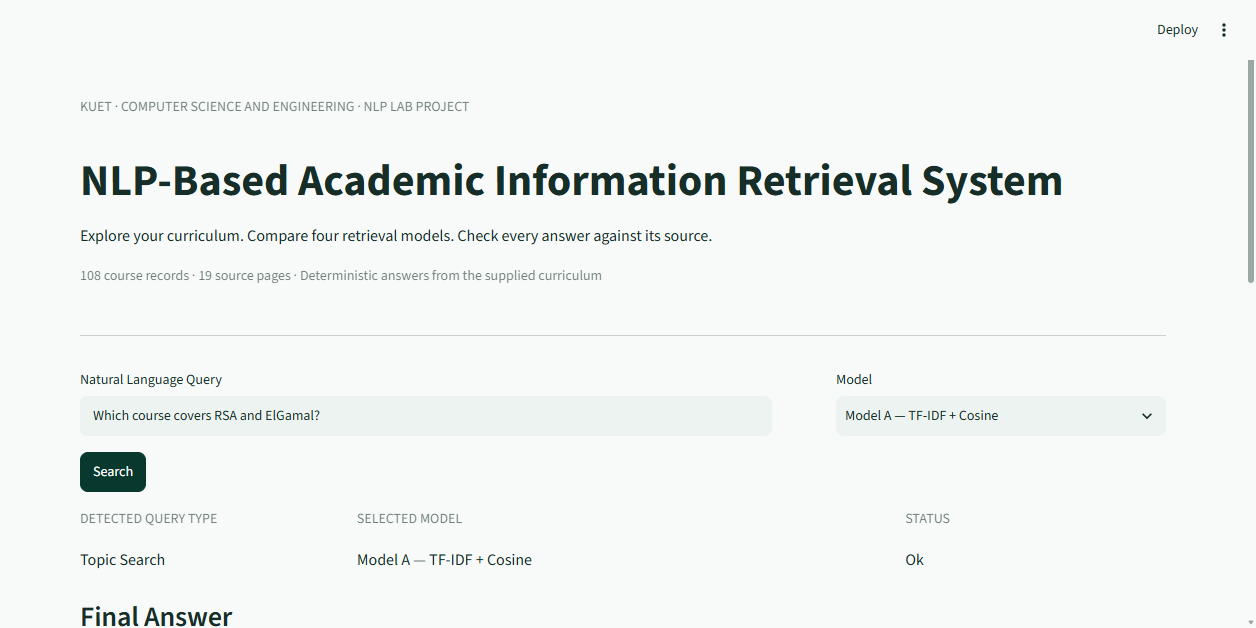
\includegraphics[width=0.9\textwidth]{figures/demo-search.png}
    \caption{Interactive Streamlit Interface Displaying Natural Language Query Results}
    \label{fig:demo_search}
\end{figure}

\subsection{Key Interface Features}
\begin{enumerate}
    \item \textbf{Two-Column Header:} A search input on the left and a model selector dropdown on the right with exact labels (\textit{``Model A --- TF-IDF + Cosine''}, \textit{``Model B --- Pretrained Word2Vec''}, \textit{``Model C --- Word2Vec + BiLSTM''}, \textit{``Model D --- Sentence-BERT''}).
    \item \textbf{Instant Model Switching:} Selecting a different model from the dropdown immediately re-evaluates the query through the new model without clearing the input or requiring manual resubmission.
    \item \textbf{Results Presentation:} Displays detected intent, selected model, status, final answer, confidence/relevance score, and a structured Top-3 table with course codes, credits, terms, and optional groups.
    \item \textbf{Source Traceability:} Expandable drawers display matched syllabus excerpts, physical PDF page numbers, and any detected metadata discrepancies.
    \item \textbf{Viva Demonstration Expander (``Show Processing Details''):}
    \begin{itemize}
        \item \textbf{Model A:} Displays preprocessed tokens and top TF-IDF matched terms with weights.
        \item \textbf{Model B:} Displays covered Word2Vec tokens and OOV tokens.
        \item \textbf{Model C:} Displays predicted relevance probability and tensor diagnostics.
        \item \textbf{Model D:} Displays embedding dimensions (384) and cosine similarities.
    \end{itemize}
\end{enumerate}

\subsection{Caching and Performance Architecture}
To achieve instantaneous query responses:
\begin{itemize}
    \item \texttt{@st.cache\_resource} keeps heavy model weights (Word2Vec vectors, BiLSTM parameters, SBERT transformer) resident in RAM.
    \item Document embeddings are precomputed once on disk.
    \item Queries are evaluated via live, real-time inference on the fly.
\end{itemize}

% ---------------------------------------------------------------------------
% CHAPTER 6: EMPIRICAL EVALUATION & RESULTS
% ---------------------------------------------------------------------------
\chapter{Empirical Evaluation and Results}

\section{Evaluation Methodology}
Evaluation was conducted on the held-out benchmark of 48 queries in \texttt{data/queries/evaluation\_queries.csv}. 

\subsection{Metrics}
\begin{itemize}
    \item \textbf{Hit@1:} Proportion of answerable queries where the gold course is ranked 1st.
    \item \textbf{Hit@3:} Proportion where a gold course appears in the top 3 ranks.
    \item \textbf{Mean Reciprocal Rank (MRR):} Average of reciprocal ranks of the first relevant document:
    \begin{equation}
        \text{MRR} = \frac{1}{|Q|} \sum_{i=1}^{|Q|} \frac{1}{\text{rank}_i}
    \end{equation}
    \item \textbf{Recall@3:} Proportion of all acceptable gold courses retrieved in the top 3 positions.
    \item \textbf{OOD Accuracy:} Accuracy in correctly rejecting out-of-domain queries.
    \item \textbf{False Acceptance Rate (FAR) \& False Rejection Rate (FRR):} Error rates on negative and positive queries, respectively.
\end{itemize}

\subsection{Evaluation Modes}
Two evaluation regimes are recorded:
\begin{enumerate}
    \item \textbf{Retrieval-Only:} Evaluates raw vector ranking prior to metadata routing or threshold rejection.
    \item \textbf{End-to-End:} Evaluates the complete system response including metadata routing and calibrated rejection.
\end{enumerate}

\section{Comparative Performance}
Table~\ref{tab:comparison_results} presents the quantitative comparison of all four models across the 48-query held-out benchmark.

\begin{table}[H]
    \centering
    \caption{Comprehensive Benchmark Evaluation on 48 Held-Out Queries}
    \label{tab:comparison_results}
    \begin{tabularx}{\textwidth}{lcrrrrrr}
        \toprule
        \textbf{Model} & \textbf{Mode} & \textbf{Hit@1} & \textbf{Hit@3} & \textbf{MRR} & \textbf{Recall@3} & \textbf{OOD Acc.} & \textbf{FAR} \\
        \midrule
        \textbf{Model A (TF-IDF)} & Retrieval-Only & 66.7\% & \textbf{91.7\%} & 0.794 & \textbf{81.4\%} & 100.0\% & 8.3\% \\
        & End-to-End & 75.0\% & 77.8\% & 0.764 & 68.7\% & 100.0\% & \textbf{0.0\%} \\
        \midrule
        \textbf{Model B (Word2Vec)} & Retrieval-Only & 61.1\% & 75.0\% & 0.707 & 65.9\% & 80.0\% & 25.0\% \\
        & End-to-End & 80.6\% & 83.3\% & 0.819 & 73.8\% & 100.0\% & 8.3\% \\
        \midrule
        \textbf{Model C (BiLSTM)} & Retrieval-Only & 5.6\% & 19.4\% & 0.183 & 16.7\% & 80.0\% & 41.7\% \\
        & End-to-End & 33.3\% & 36.1\% & 0.347 & 31.0\% & 100.0\% & 16.7\% \\
        \midrule
        \textbf{Model D (SBERT)} & Retrieval-Only & \textbf{77.8\%} & 86.1\% & \textbf{0.818} & 78.4\% & 100.0\% & 25.0\% \\
        & End-to-End & \textbf{83.3\%} & \textbf{88.9\%} & \textbf{0.856} & \textbf{79.1\%} & 100.0\% & \textbf{0.0\%} \\
        \bottomrule
    \end{tabularx}
\end{table}

\section{Category-Specific Analysis}
Table~\ref{tab:category_results} breaks down End-to-End Hit@1 accuracy by query category.

\begin{table}[H]
    \centering
    \caption{End-to-End Hit@1 Accuracy Across Query Categories}
    \label{tab:category_results}
    \begin{tabularx}{\textwidth}{lrrrr}
        \toprule
        \textbf{Query Category (Count)} & \textbf{Model A} & \textbf{Model B} & \textbf{Model C} & \textbf{Model D} \\
        \midrule
        Exact Terminology (12) & 75.0\% & 50.0\% & 8.3\% & 66.7\% \\
        Semantic Paraphrase (9) & 44.4\% & \textbf{88.9\%} & 11.1\% & 77.8\% \\
        Typo-Infused (3) & \textbf{100.0\%} & \textbf{100.0\%} & 66.7\% & \textbf{100.0\%} \\
        Partial Query (2) & \textbf{100.0\%} & \textbf{100.0\%} & 0.0\% & \textbf{100.0\%} \\
        Metadata Inquiries (7) & \textbf{100.0\%} & \textbf{100.0\%} & \textbf{100.0\%} & \textbf{100.0\%} \\
        Ambiguous Keywords (3) & 66.7\% & \textbf{100.0\%} & 33.3\% & \textbf{100.0\%} \\
        Out-of-Domain Rejection (5) & \textbf{100.0\%} & \textbf{100.0\%} & \textbf{100.0\%} & \textbf{100.0\%} \\
        \bottomrule
    \end{tabularx}
\end{table}

\section{Discussion and Academic Findings}
\subsection{Strengths of Sentence-BERT (Model D)}
Sentence-BERT delivers the highest top-1 accuracy (83.3\% End-to-End) and MRR (0.856). Its transformer attention layers effectively capture syntactic semantics and sentence composition, excelling on both semantic queries and partial phrases.

\subsection{The Enduring Power of TF-IDF (Model A)}
For exact academic terminology (e.g., \textit{``BLAST''}, \textit{``Amdahl's law''}, \textit{``RSA''}), Model~A performs remarkably well, achieving the highest raw Hit@3 (91.7\%). When specialized vocabulary matches the syllabus, lexical counting remains an exceptionally competitive, zero-overhead baseline.

\subsection{Critical Analysis of Model C (BiLSTM Overfitting)}
Model~C achieves only 5.6\% raw Hit@1 and 19.4\% Hit@3 on the held-out benchmark. This is an important, honest scientific finding:
\begin{itemize}
    \item \textbf{Data Scarcity:} The training set comprised 68 queries and 398 sampled pairs. Deep recurrent architectures with dense interaction layers have large parameter spaces that rapidly overfit on small sample sets.
    \item \textbf{Loss Divergence:} Training loss dropped consistently to near zero while validation loss plateaued at epoch 12 ($0.5127$), typical of over-parameterized neural networks memorizing small training sets.
    \item \textbf{Curricular Lesson:} Pretrained foundation embeddings (Models B and D) vastly outperform small supervised neural models trained from scratch when labeled domain data is scarce. This result is preserved as an authentic comparative finding in the report.
\end{itemize}

% ---------------------------------------------------------------------------
% CHAPTER 7: VERIFICATION & TESTING
% ---------------------------------------------------------------------------
\chapter{Automated Testing and Verification}

\section{Test Architecture}
The codebase includes a comprehensive automated test suite in the \texttt{tests/} directory, executed via \texttt{pytest}. All 29 unit and integration tests pass successfully without errors.

\section{Verification Coverage}
\begin{itemize}
    \item \textbf{Corpus Completeness (\texttt{test\_core.py}):} Validates that all 108 records and 107 unique codes are extracted, with no null credits or missing contact hours.
    \item \textbf{Formatting Edge Cases:} Asserts that syllabus continuations across page boundaries and missing colons (e.g., \texttt{CSE 4245}) are correctly parsed.
    \item \textbf{Typo and Normalization Testing:} Verifies that code variations (\texttt{CSE4121}, \texttt{CSE-4121}) map to standard forms and that edit-distance correctly replaces misspelled academic words.
    \item \textbf{Rejection Verification:} Confirms that empty inputs, gibberish strings, out-of-domain inquiries, and unsupported fields return exact rejection statuses.
    \item \textbf{Year/Term and Lab Inquiries:} Tests multi-record retrieval for 4th year labs (15 courses), term-specific sessionals, and theory filtering.
    \item \textbf{Neural Verification (\texttt{test\_neural.py}):} Verifies packed sequence padding invariance, OOV token masking, and synthetic gradient learning in the BiLSTM.
    \item \textbf{Streamlit UI Testing (\texttt{test\_app.py}):} Utilizes Streamlit's headless testing framework (\texttt{AppTest}) to verify button interactions, live model switching, and graceful fallback when Model~D is disabled via environment variables.
\end{itemize}

% ---------------------------------------------------------------------------
% CHAPTER 8: CONCLUSION & FUTURE SCOPE
% ---------------------------------------------------------------------------
\chapter{Conclusion and Future Work}

\section{Summary of Contributions}
This project successfully designed and implemented an academic Information Retrieval system for the KUET CSE undergraduate curriculum. By strictly adhering to zero-hallucination, non-generative constraints, the system provides grounded, verifiable academic search with source page citations.

The work directly synthesizes the five laboratory modules of the NLP curriculum into an end-to-end operational software product:
\begin{itemize}
    \item Established an automated extraction and conflict-auditing pipeline for institutional curriculum PDFs.
    \item Built and benchmarked four distinct NLP paradigms: TF-IDF, Word2Vec, BiLSTM, and Sentence-BERT.
    \item Conducted an honest, reproducible comparative evaluation demonstrating the strengths of transformer contextual embeddings and the data-scarcity failure modes of small supervised deep learning models.
    \item Delivered an interactive, high-performance Streamlit application with explainable scoring diagnostics and instantaneous model switching.
\end{itemize}

\section{Future Work}
Future directions for expanding this research include:
\begin{enumerate}
    \item \textbf{Expanded Supervised Data:} Crowd-sourcing or student-annotating thousands of query-course relevance pairs to investigate the data threshold at which supervised BiLSTMs become competitive.
    \item \textbf{Hybrid Dense-Lexical Search:} Developing reciprocal rank fusion (RRF) combining Model~A (for rare technical acronyms) and Model~D (for semantic intent).
    \item \textbf{Cross-Departmental Scaling:} Extending the PDF parser and corpus builder to ingest curricula from other engineering departments across KUET.
\end{enumerate}

% ---------------------------------------------------------------------------
% REFERENCES
% ---------------------------------------------------------------------------
\begin{thebibliography}{99}
\bibitem{manning2008} C. D. Manning, P. Raghavan, and H. Schütze, \textit{Introduction to Information Retrieval}, Cambridge University Press, 2008.
\bibitem{mikolov2013} T. Mikolov, I. Sutskever, K. Chen, G. S. Corrado, and J. Dean, ``Distributed representations of words and phrases and their compositionality,'' \textit{Advances in Neural Information Processing Systems (NeurIPS)}, vol. 26, 2013.
\bibitem{reimers2019} N. Reimers and I. Gurevych, ``Sentence-BERT: Sentence embeddings using Siamese BERT-networks,'' \textit{Proceedings of the 2019 Conference on Empirical Methods in Natural Language Processing (EMNLP)}, 2019.
\bibitem{hochreiter1997} S. Hochreiter and J. Schmidhuber, ``Long short-term memory,'' \textit{Neural Computation}, vol. 9, no. 8, pp. 1735--1780, 1997.
\bibitem{pymupdf} Artifex Software, ``PyMuPDF Documentation,'' \url{https://pymupdf.readthedocs.io/}, 2024.
\bibitem{scikit-learn} F. Pedregosa et al., ``Scikit-learn: Machine learning in Python,'' \textit{Journal of Machine Learning Research}, vol. 12, pp. 2825--2830, 2011.
\bibitem{streamlit} Streamlit Inc., ``Streamlit Documentation and Testing Framework,'' \url{https://docs.streamlit.io/}, 2024.
\end{thebibliography}

\end{document}
